\documentclass[../main.tex]{subfiles}

\begin{document}
	Nella paragrafo predente abbiamo definito l'operazione di Trasformata di Laplace:
	$$\Lapl{f(t)\ \text{definita in}\ \left[ 0^-;+\infty \right]}{F(s)=\Lbrace{f(t)}}  $$
	Se vogliamo effettuare l'operazione inversa della trasformata:
	$$ \aLapl{ \Lapl{f(t)}{F(s)} }{ \tilde{f}(t) } $$
	Ci aspettiamo che: 
	$$ \tilde{f}(t) \equiv f(t) \quad \forall t \in \left[ 0^-;+\infty \right] $$
	%esempio e grafici
	\linebreak
	Data una funzione $ F(s)\: s \in \C\: $ con caratteristiche tali da poter essere considerata una \hyperref[sec:traformata_laplace]{trasfromata di Laplace} (continuit\'{a}, derivabilit\'{a} per tutti gli ordini, ascissa di convergenza ...) di una funzione $ f(t) $, allora vorremmo trovare $ f(t) $ almeno (solo) in $ \left[ 0^-;+\infty \right) $ (cio\'{e} trovare $ f(t) \cdot 1(t) $).\\
	\linebreak
	Senza dimostrare, la formula generale dell'anti-trasformata di Laplace \'{e}:
	\[ \aLbrace{F(s)} = \frac{1}{j2\pi} \int_{ \ncompl{\sigma}{\infty} }^{ \compl{\sigma}{\infty} } F(s) e^{st} \mathrm{d}s \qquad \sigma > \bar{\sigma} \quad \text{ascissa di convergenza} \]
	Questa formula non la useremo mai, ma cercheremo di calcolarle sfruttando le \hyperref[subsec:prop_laplace]{propriet\'{a}} della trasformata.
	\[ F(s) = \Lbrace{f(t)} \quad \Rightarrow \quad \aLbrace{F(s)} = f(t) \cdot 1(t) \]
	\'{E} importante ricordarsi sempre di mettere 1(t) nell'anti-trasformata perch\'{e} non consideriamo cosa \'{e} successo prima di zero. Se non lo mettiamo facciamo un errore perch\'{e} troviamo l'anti-trasformata di una funzione diversa. 
	%
	\section{Esempi introduttivi}
	\begin{enumerate}
		\item $ \quad \aLbrace{\dfrac{1}{s}} = 1 \cdot 1(t) $
		\item $ \quad \aLbrace{\frac{1}{s-2}} = e^{2t} 1(t) \qquad \text{\hyperref[trasl_s]{traslazione in s}}$
		\item $ \quad \aLbrace{\dfrac{1}{s+2}} = e^{-2t} 1(t) \qquad \text{\hyperref[trasl_s]{traslazione in s}}$
		\item $ \quad \aLbrace{\dfrac{1}{s^2}} = \left. \dfrac{1}{n!} t^n 1(t) \right|_{n=1} = t \cdot 1(t) \qquad \text{\hyperref[deriv_n_t]{derivata n-esima in t}}$\\
		\linebreak
		In generale:
		\[ \aLapl{\frac{1}{s^m}}{\frac{1}{(m-1)!} t^{m-1} \cdot 1(t)} \]
		\item $ \quad \aLbrace{\frac{1}{(s-a)^m}} = \aLbrace{ \left. \frac{1}{\bar{s}^{m}} \right|_{\bar{s} = s-a}} = \frac{1}{(m-1)!} t^{m-1} e^{at} 1(t) \qquad \text{\hyperref[trasl_s]{traslazione in s}} $
		\item $ \quad \aLbrace{\frac{3}{s^2+4s+13}} = ? $\\
		\linebreak
		Completiamo i quadrati del denominatore:
		\[ s^2+4s+13 = s^2+2 \cdot (\color{red}2\color{black}s) \color{red}+ 2^2 - 2^2\color{black} +9 = (s+2)^2+(3)^2 \]
		In generale se abbiamo un polinomio di secondo grado del tipo:
		\[ \left[ s-(\compl{\sigma}{w}) \right] \left[ s-(\ncompl{s}{w}) \right] = \left[ (s-\sigma) \compl{}{w}\right] \left[ (s-\sigma) \ncompl{}{w}\right] = (s-\sigma)^2 + w^2 \]
		Ha come radici $ \qquad \sigma \pm jw $\\
		\linebreak
		Quindi nel nostro caso $ \qquad \sigma=-2 \quad w=3 $
		\[ \aLbrace{\frac{3}{(s+2)^2+9}} = e^{-2t} \sin(3t) 1(t) \]
		\item $ \quad \aLbrace{\frac{12}{(s+2)^2+9}} = 4 \cdot \aLbrace{\frac{3}{(s+2)^2+9}} = 4e^{-2t} \sin(3t) 1(t) $
		\item $ \quad \aLbrace{\frac{s+2}{(s+2)^2+9}} = e^{-2t} \cos(3t) 1(t) $
		\item $ \quad \aLbrace{\frac{s+5}{s^2+4s+13}} = \aLbrace{\frac{s+2}{(s+2)^2+9} + \frac{3}{(s+2)^2+9}} = e^{-2t} \left[ cos(3t)+sin(3t) \right] 1(t)$
		\item $ \quad \aLbrace{e^{-4s} \frac{3}{(s+2)^2+9}} = ? $
		\[ \aLapl{\frac{3}{(s+2)^2+9}}{e^{-2t} \sin(3t) 1(t)} \]
		L'esponenziale in s comporta una \hyperref[trasl_t]{traslazione in t}:
		\[ \Lapl{f(t-T) 1(t-T)}{e^{-sT} F(S)} \]
		\[ \aLapl{e^{-4s} \frac{3}{(s+2)^2+9}}{e^{-2(t-4)} \sin \left[ 3(t-4) \right] 1(t-4)} \]
		Quindi otteniamo in generale:
		\[ \aLapl{F(s) e^{-sT}}{f(t-T)1(t-T)} \]
	\end{enumerate}
	%
	\section{Funzioni razionali}
	\[ F(s) = \frac{b_m s^m + b_{m-1} s^{m-1} + _{\dots} + b_1 s + b_0}{a_n s^n + a_{n-1} s^{n-1} + _{\dots} + a_1 s + a_0 } = \frac{A(s)}{B(s)} \]
	Supponiamo che $ a_n \neq 0, b_m \neq 0 $ cos\'{\i} $m$ e $n$ sono effettivamente i gradi dei polinomi: 
	$$ m = \deg\left\lbrace B(s) \right\rbrace, n=\deg \left\lbrace A(s) \right\rbrace $$
	\begin{align*}
		n \geq m \quad &\Rightarrow \quad F(s) \quad \text{\textbf{propria}}\\
		n > m \quad &\Rightarrow \quad F(s) \quad \text{\textbf{strettamente} propria}\\
		n = m \quad &\Rightarrow \quad F(s) \quad \text{\textbf{semplicemente} propria}
	\end{align*}
	%
	\subsection{Fattorizzazione di un polinomio}
	\[ F(s) = \frac{B(s)}{A(s)} = \frac{b_m}{a_n} \frac{(s-z_1)^{m_1}\: _{\dots}\: (s-z_h)^{m_h}}{(s-p_1)^n\: _{\dots}\: (s-p_k)^{n_k}} \]
	\begin{align*}
		&z_1, z_2, \dots z_h \quad &&\text{sono gli ZERI (le radici distinte di B(s))}\\
		&p_1, p_2, \dots p_k \quad &&\text{sono i POLI (le radici distinte di A(s))}\\
		&m_1, m_2, \dots m_h \quad &&\text{sono le molteplicit\'{a} degli zeri} \Rightarrow \sum_{i=1}^{h}m_i = m\\
		&n_1, n_2, \dots n_k \quad &&\text{sono le molteplicit\'{a} dei poli} \Rightarrow \sum_{i=1}^{k}n_i = n\\
	\end{align*}
	\section{Funzione razionale strettamente propria}
	\begin{align*}
		F(s) = \frac{B(s)}{A(s)} &= c_{1,1} \frac{1}{(s-p_1)} + c_{1,2} \frac{1}{(s-p_1)^2} + \dots + c_{1,n_1} \frac{1}{(s-p_1)^{n_1}} +\\
		&+ c_{2,1} \frac{1}{(s-p_2)} + \dots + c_{2,n_2} \frac{1}{(s-p_2)^{n_2}} + \dots + \\
		&+ c_{k,1} \frac{1}{(s-p_k)} + \dots + c_{k,n_k} \frac{1}{(s-p_k)^{n_k}} =\\
		&= \sum_{i=1}^{k} \sum_{j=1}^{n_i} c_{i,j} \frac{1}{(s-p_i)^j}
	\end{align*}
	$c_{i,j}$ dove $i$ indica il polo, mentre $j$ indica la molteplicit\'{a} del polo. Ma come calcolare questi coefficienti?\\
	\begin{itemize}
		\item Concentriamoci sul polo $p_l$ con molteplicit\'{a} $n_l$. Quindi calcoliamo:
		\begin{align*}
			(s-p_l)^{n_l} F(s) = (s-p_l)^{n_l} \cdot \left( \sum_{i \neq l} \sum_{j=1}^{n_i} c_{i,j} \frac{1}{(s-p_i)^j} \right) &+ c_{l,1} (s-p_l)^{n_l -1} + c_{l,2} (s-p_l)^{n_l -2} + \dots +\\
			&+ c_{l,n_l -1} (s-p_l)^{n_l - (n_l -1)} + c_{l,n_l}
		\end{align*}
		Calcolando questa espressione in $p_l$ tutti i termini si annullano tranne uno:
		\[ c_{l,n_l} = \left. (s-p_l)^{n_l} \cdot F(s) \right|_{s=p_l} \]
		\item Deriviamo l'espressione e calcoliamola in $p_l$:
		\[ c_{l,n_l-1} = \left. \der{}{s} (s-p_l)^{n_l} \cdot F(s) \right|_{s=p_l} \]
		\linebreak
		\[ \dots \]
		\linebreak
		\item Continuando a derivare stando attenti ai coefficienti dovuti alla derivazione:
		\begin{equation}
		\label{residuo}
			c_{l,q} = \left. \frac{1}{(n_l - q)!}\: \der{{}^{n_l - q}}{s^{n_l - q}} (s-p_l)^{n_l} \cdot F(s) \right|_{s=p_l} \quad \in \C
		\end{equation}
		L'espressione \ref{residuo} \'{e} detta \textbf{residuo q-esimo} del polo l-esimo, dove:
		\begin{itemize}
			\item $ p_l $ \'{e} l'l-esimo polo
			\item $ n_l $ \'{e} la molteplicit\'{a} dell'l-esimo polo
			\item $ l $ \'{e} l'indice del residuo: varia tra $ 1 $ e $ n_l $
		\end{itemize}
	\end{itemize}
	%
	\subsection{Esempio di residui complessi}
	\[ \frac{1}{s^2+4} = c_{1,1} \frac{1}{\ncompl{s}{2}} + c_{2,1} \frac{1}{\compl{s}{2}} \qquad p_1 = 2j,\quad p_2 = -2j\]
	Usiamo la formula \ref{residuo} per il primo coefficiente dove $ n_l = 1 \quad q = 1 $:
	\begin{itemize}
		\item $ p_1 = 2j $:
		\[ 
			c_{1,1} = \left. \frac{1}{(1-1)!} \cdot (s-2j) \cdot \frac{1}{(s-2j)(s+2j)} \right|_{s=2j} = \left. \frac{1}{s+2j} \right|_{s=2j} = \frac{1}{4j}
		\]
		\item $ p_2 = -2j $:
		\[ 
			c_{2,1} = \left. \frac{1}{(1-1)!} \cdot (s+2j) \cdot \frac{1}{(s-2j)(s+2j)} \right|_{s=2j} = \left. \frac{1}{s-2j} \right|_{s=2j} = \frac{1}{-4j}
		\]
	\end{itemize}
	%
	\subsection{Esempio di residui reali}
	\[ \frac{s}{s^2-1} \qquad p_1 = -1\ (n_1 = 1) \qquad p_2 = 1\ (n_2 = 1) \]
	\[ \frac{s}{s^2-1} = \frac{c_{1,1}}{s+1}  + \frac{c_{2,1}}{s-1} = \frac{c_{1,1}(s-1) + c_{2,1}(s+1)}{s^2-1} = \frac{(c_{1,1} + c_{2,1})s + (c_{2,1} - c_{1,1})}{s^2-1} \]
	\[ \begin{cases}
		c_{1,1} + c_{2,1} &= 1\\
		c_{1,1} &= c_{2,1}
	\end{cases}
	\qquad \Rightarrow \qquad c_{1,1} = c_{2,1} = \frac{1}{2} \]
	\[ \frac{s}{s^2-1} = \frac{1}{2} \frac{1}{s+1} + \frac{1}{2} \frac{1}{s-1} \]
	%
	\section{Generalizzazione dei fratti semplici}
	In generale data una funzione razionale $ F(s) = \frac{B(s)}{A(s)}$ strettamente propria a coefficienti reali, dove le radici di $ A(s) $ sono:
	\begin{itemize}
		\item $ p_1\ \dots\ p_r $ \quad poli reali distinti
		\item $ n_1\ \dots\ n_r $ \quad molteplicit\'{a} dei poli reali
		\item $ \bar{p}_1\ \dots\ \bar{p}_c $ \quad coppie coniugate di poli complessi
		\item $ \bar{n}_1\ \dots\ \bar{n}_c $ \quad molteplicit\'{a} dei poli complessi
		\item $ c_{i,l},\; \bar{c}_{i,l}^{\ \sin},\; \bar{c}_{i,l}^{\ \cos} \in \mathbb{R} $
	\end{itemize}
	\begin{align}
		F(s) = \frac{B(s)}{A(s)} &= \sum_{i=1}^{r} \sum_{l=1}^{n_i} c_{i,l} \frac{1}{(s-p_i)^l} +\\
		&+ \sum_{i=1}^{c} \sum_{l=1}^{\bar{n}_i} \left[ \bar{c}_{i,l}^{\ \sin} \frac{\text{Polinomio}_{i,l}^{\sin}(s)}{[(s - \sigma_i)^2 + w_i^2]^l} + \bar{c}_{i,l}^{\ \cos} \frac{\text{Polinomio}_{i,l}^{\cos}(s)}{[(s - \sigma_i)^2 + w_i^2]^l} \right]
	\end{align}
	Bisogna notare che i poli complessi essendo coniugati sono \textit{spariti} svolgendo qualche passaggio matematico.\\
	Ad esempio in un polinomio di secondo grado con due radici complesse $ p_1 = \sigma + jw $ e $ p_2 = \sigma - jw $:
	\[ (s - p_1)(s - p_2) = [s - (\sigma + jw)][s - (\sigma - jw)] =  \]
	\[ = [(s - \sigma) - jw][(s - \sigma) + jw] = (s - \sigma)^2 + w^2 \]
	%
	Quindi possiamo distinguere due gruppi:
	\begin{itemize}
		\item i fratti semplici a \textbf{poli reali} si antitrasformano essenzialmente con degli esponenziali. Se i poli hanno una molteplicit\'{a} maggiore di uno, allora compariranno anche dei polinomi:
		\[ \aLapl{(2.4)}{c_{i,l} \frac{1}{(l-1)!} t^{l-1} e^{p_i t} 1(t)} \]
		\item i fratti semplici a \textbf{poli complessi} invece si antitrasformano con seni e coseni:
		\[ \aLapl{(2.5)}{e^{\sigma t} sin(wt) \cdot [A_1 + A_2 t + A_3 t^2 + \dots] \quad + \quad e^{\sigma t} cos(wt) \cdot [B_1 + B_2 t + B_3 t^2 + \dots]} \]
	\end{itemize}
	%
	\subsection{Osservazioni}
	(IMPORTANTE) Se non esistono semplificazioni tra numeratore e denominatore (non esiste una radice comune tra i due), allora i residui relativi ai fratti semplici di grado massimo per ciascun polo sono diversi da zero.
	%
	\subsection{Esempio di poli complessi}
	$ \quad \aLbrace{\frac{3s+10}{s^2+4s+13}} = ? $\\
	\linebreak
	Dobbiamo scomporre la funzione razionale in fratti semplici. In generale:
	\[ \frac{as+b}{(s-\sigma)^2 + w^2} = A \frac{w}{(s-\sigma)^2 + w^2} + B \frac{(s-\sigma)}{(s-\sigma)^2 + w^2} = \frac{Aw +Bs- B\sigma}{(s-\sigma)^2 + w^2}\]
	\begin{itemize}
		\item Riscriviamo la funzione razionale come combinazione lineare di funzioni razionali in cui a numeratore abbiamo un polinomio di grado 0 e uno di grado 1. Con una combinazione lineare di un qualsiasi polinomio di grado 0 con un polinomio di grado 1, possiamo scrivere un qualsiasi polinomio di grado 1, come quello di partenza $as+b$.
		\item Attraverso il principio di uguaglianza fra polinomi (due polinomi sono uguali se i coefficienti omologhi sono uguali) confrontiamo il nuovo polinomio $ Aw +Bs- B\sigma $ con quello di partenza $as+b$.
		\item Quindi alla fine dobbiamo risolvere un sistema lineare di due equazioni in 2 incognite con un unica soluzione perch\'{e} ha rango massimo:  
		$\begin{cases}B &= a\\Aw + B\sigma &= b\end{cases}$
	\end{itemize}
	Quindi nel nostro esempio otteniamo:
	\[ \frac{3s+10}{s^2+4s+13} = A\frac{3}{(s+2)^2+9} + B\frac{s+2}{(s+2)^2+9} = \frac{3A + Bs + 2B}{(s+2)^2+9} \]
	\[ 
	\begin{cases} B &= 3\\ 3A + 2B &= 10\end{cases} \qquad
	\begin{cases} B &= 3\\ A &= \frac{4}{3}\end{cases} 
	\]
	\[ \Rightarrow \frac{4}{3} \frac{3}{(s+2)^2+9} + 3 \frac{s+2}{(s+2)^2+9} \]
	\[ \aLapl{}{\frac{4}{3} e^{-2t} \sin(3t) 1(t) + 3 e^{-2t} \cos(3t) 1(t) } \]
	%
	\subsection{Esempio di poli complessi 2}
	Bisogna utilizzare la trasformata in $ s $ del polinomio + esponenziale + sinusoide:
	\begin{align*}
		\frac{\text{polinomio grado}\: \leq 3}{[(s-3)^2 + 4]^2} &= A \frac{2}{(s-3)^2 + 4} + B \frac{s - 3}{(s-3)^2 + 4} +\\
		&+ C \frac{4 \cdot (s-3)}{[(s-3)^2 + 4]^2} + D \frac{(s - 3)^2 - 4}{[(s-3)^2 + 4]^2}
	\end{align*}
	Dopo aver risolto un sistema per trovare i quattro coefficienti, l'anti-trasformata \'{e}:
	\[ f(t) = e^{3t} [A \sin(2t) + B \cos(2t) + t\ C \sin(2t) + t\ D \cos(2t)] \]
	%
	\section{Funzione razionale propria}
	Partiamo con un esempio di una funzione propria: $ \pDeg{B(s)} \geq \pDeg{A(s)} $
	\[ F(s) = \frac{B(s)}{A(s)} = \frac{s^2+1}{s^2-1} \]
	Effettuiamo la divisione tra i due polinomi:
	\[ 
	\begin{array}{ccc|c}
	s^2 & +1 & & s^2-1\\ \cline{4-4}
	s^2 & -1 & & 1\\ \cline{1-2}
	0 	& 2  & &
	\end{array}
	 \]
	Ci fermiamo nella divisione quando raggiungiamo l'ultimo termine con potenza positiva o nulla (come in questo caso). Se avessimo continuato, avremmo ottenuto termini con potenze negative.
	\[ \frac{B(s)}{A(s)} = \frac{s^2+1}{s^2-1} = Q(s) + \frac{R(s)}{A(s)} = 1 + \frac{2}{s^2-1} \]
	dove $ Q(s) $ \'{e} il polinomio \textit{quoziente}, $ R(s) $ il polinomio resto.
	A secondo membro abbiamo ottenuto una funzione razionale strettamente propria. Quindi applichiamo i fratti semplici:
	\[ \frac{2}{s^2-1} = \frac{A}{s+1} + \frac{B}{s-1} = \frac{A(s-1) + B(s+1)}{s^2-1} = \frac{(A+B)s + (B-A)}{s^2-1} \]
	\[ 
		\begin{cases} A + B = 0\\B - A = 0\end{cases} \quad
		\begin{cases} B = -A\\ B = 1\end{cases} \quad
		\begin{cases} A = -1\\ B = 1\end{cases}
	\]
	Quindi concludiamo l'esercizio:
	\[ \aLapl{F(s) = 1 - \frac{1}{s+1} + \frac{1}{s-1}}{ \delta(t) + (-e^{-t} + e^t) \cdot 1(t)} \]
	\rule{\linewidth}{.4pt}
	\smallskip\\
	In generale $ m \geq n, \quad m = \pDeg{B(s)} \quad n = \pDeg{A(s)} $:
	\[ F(s) = \frac{B(s)}{A(s)} = k_0 + k_1 s + k_2 s^2 + \dots + k_{m-n} s^{m-n} + \frac{\tilde{B}(s)}{A(s)} \]
	con $ \pDeg{\tilde{B}(s)} < \pDeg{A(s)} $ e quindi la frazione resto \'{e} risolvibile con i fratti semplici.
	\[ \aLapl{F(s)}{\delta(t) + \der{}{t} \delta(t) + \der{^2}{t^2} \delta(t) + \dots + \der{^{m-n}}{t^{m-n}} \delta(t) + \aLbrace{\tilde{B}(s)}{A(s)}} \]
	%
	\section{Andamento nel tempo dell'antitrasformata}
	\begin{itemize}
		\item $ \re{p} < 0 \quad \Rightarrow \quad $ l'antitrasformata tende a zero
		\item $ \re{p} = 0\ \text{e molteplicit\'{a}}\ = 1 \quad \Rightarrow \quad $ non tende a zero, ma \'{e} limitata
		\item $ \re{p} > 0\ \text{oppure}\ \re{p}\ = 0\ \text{e molteplicit\'{a}} > 1 \quad \Rightarrow \quad $ non \'{e} limitata e diverge a $ \pm \infty $
	\end{itemize}
	\rule{\linewidth}{0.4pt}
	\paragraph{Poli reali:} $ p = \sigma \in \R $
	%1
	\begin{figure}[h!]
		\centering
		\[ \aLapl{\frac{1}{s-\sigma}}{e^{\sigma t} 1(t)} \]
		\begin{subfigure}{0.3\textwidth}
			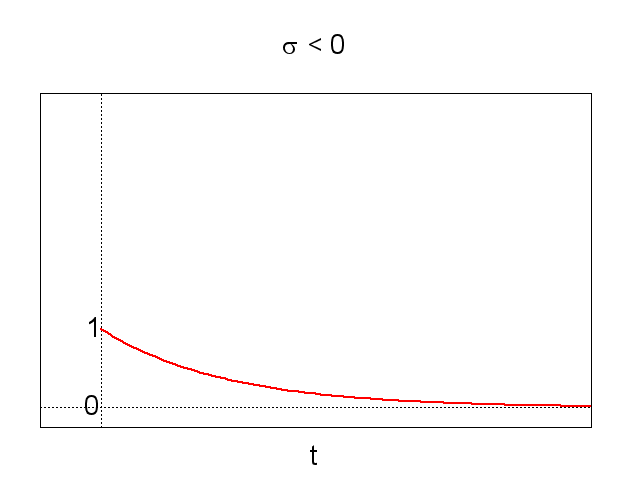
\includegraphics[width=5cm, height=4cm]{plot/andamento_t/poli_reali1_1}
		\end{subfigure}
		\begin{subfigure}{0.3\textwidth}
			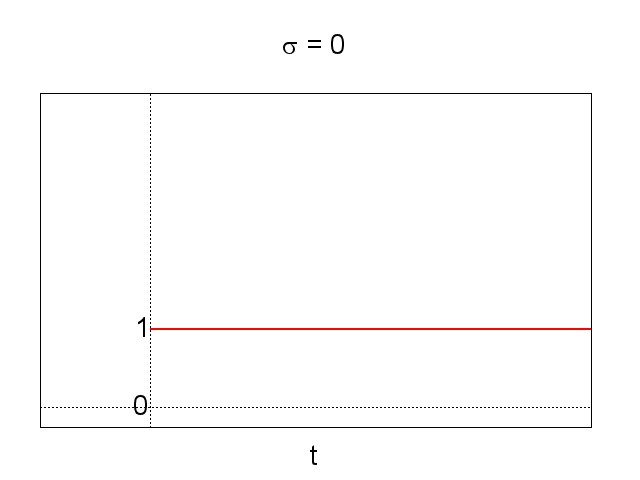
\includegraphics[width=5cm, height=4cm]{plot/andamento_t/poli_reali1_2}
		\end{subfigure}
		\begin{subfigure}{0.3\textwidth}
			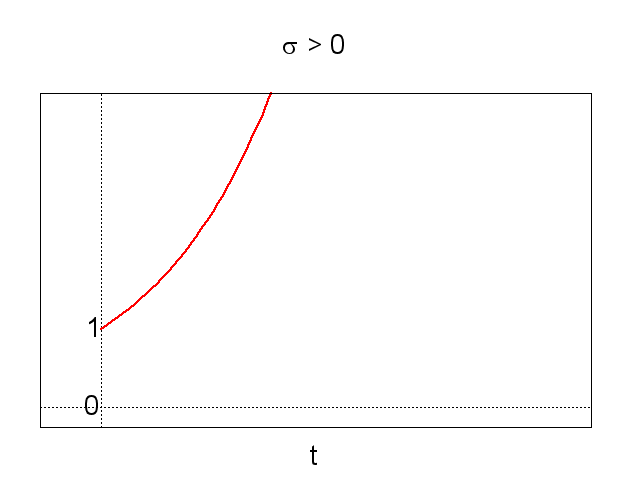
\includegraphics[width=5cm, height=4cm]{plot/andamento_t/poli_reali1_3}
		\end{subfigure}
	\end{figure}\\
	%2
	\begin{figure}[h!]
		\[ \aLapl{\frac{1}{(s-\sigma)^2}}{t e^{\sigma t} 1(t)} \]
		\centering
		\begin{subfigure}{0.3\textwidth}
			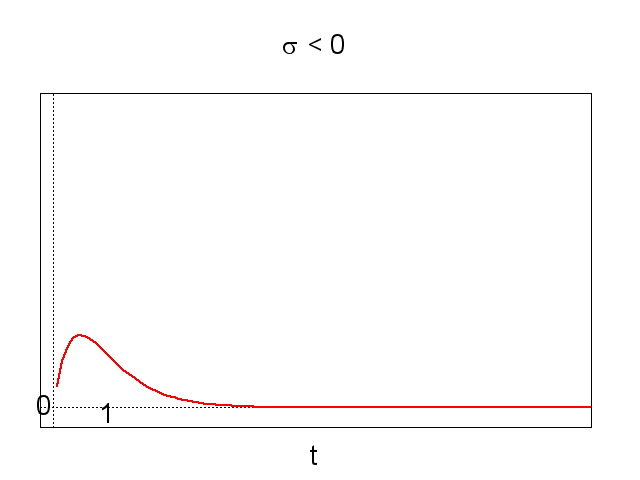
\includegraphics[width=5cm, height=4cm]{plot/andamento_t/poli_reali2_1}
		\end{subfigure}
		\begin{subfigure}{0.3\textwidth}
			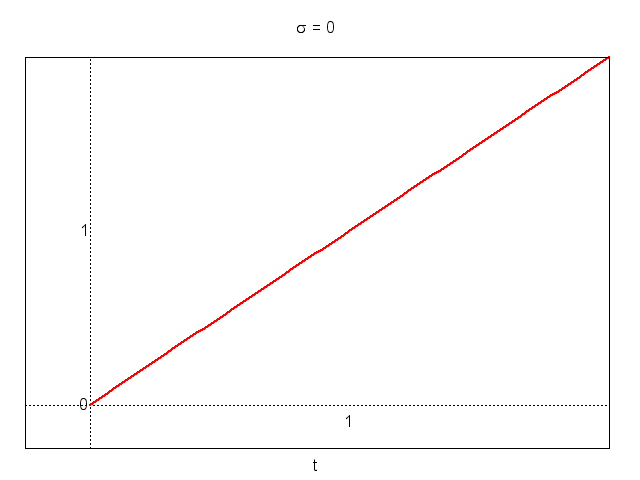
\includegraphics[width=5cm, height=4cm]{plot/andamento_t/poli_reali2_2}
		\end{subfigure}
		\begin{subfigure}{0.3\textwidth}
			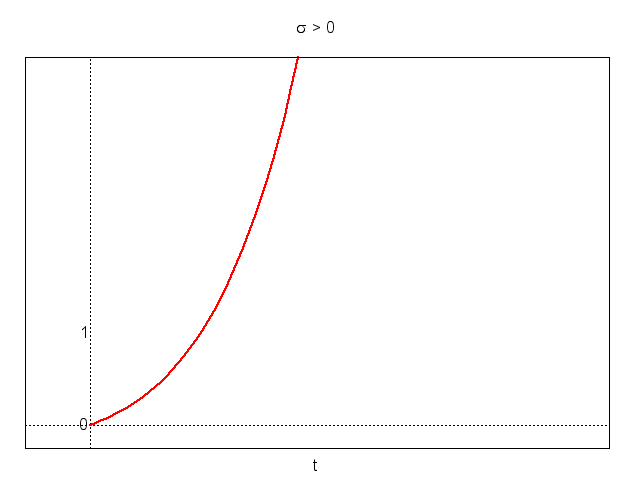
\includegraphics[width=5cm, height=4cm]{plot/andamento_t/poli_reali2_3}
		\end{subfigure}
	\end{figure}\\
	%3
	\begin{figure}[h!]
		\[ \aLapl{\frac{1}{(s-\sigma)^n}}{\frac{1}{(n-1)!} t^{n-1} e^{\sigma t} 1(t)} \]
		\centering
		\begin{subfigure}{0.3\textwidth}
			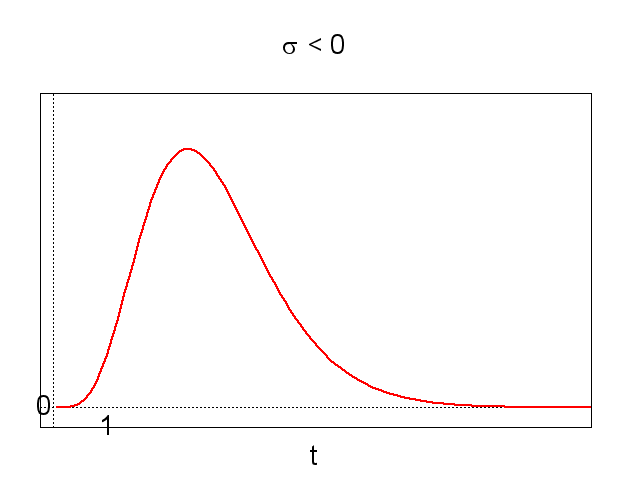
\includegraphics[width=5cm, height=4cm]{plot/andamento_t/poli_reali3_1}
		\end{subfigure}
		\begin{subfigure}{0.3\textwidth}
			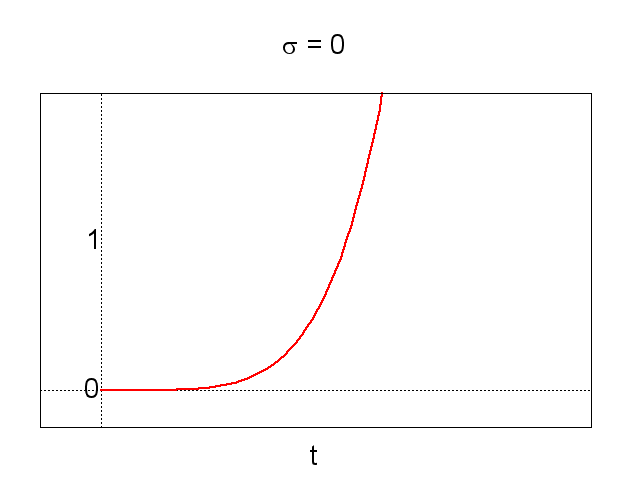
\includegraphics[width=5cm, height=4cm]{plot/andamento_t/poli_reali3_2}
		\end{subfigure}
		\begin{subfigure}{0.3\textwidth}
			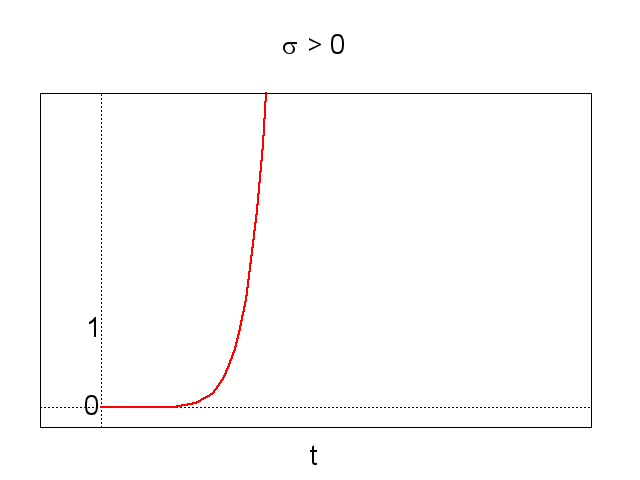
\includegraphics[width=5cm, height=4cm]{plot/andamento_t/poli_reali3_3}
		\end{subfigure}
	\end{figure}
	\newpage
	%
	\noindent
	\rule{\linewidth}{0.4pt}\\%
	\paragraph{Poli complessi:} $ p = \sigma \pm jw \quad w \neq 0 $
	%1
	\begin{figure}[h!]
		\[ \aLapl{ \frac{c}{s-p} + \frac{c^*}{s-p^*} }{ e^{\sigma t} (A \sin wt + B \cos wt) = D e^{\sigma t} \cos (wt + \phi) }  \]
		\centering
		\begin{subfigure}{0.3\textwidth}
			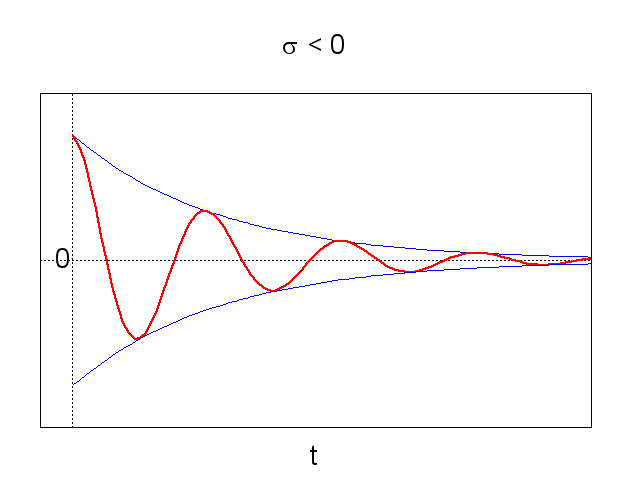
\includegraphics[width=5cm, height=4cm]{plot/andamento_t/poli_complessi1_1}
		\end{subfigure}
		\begin{subfigure}{0.3\textwidth}
			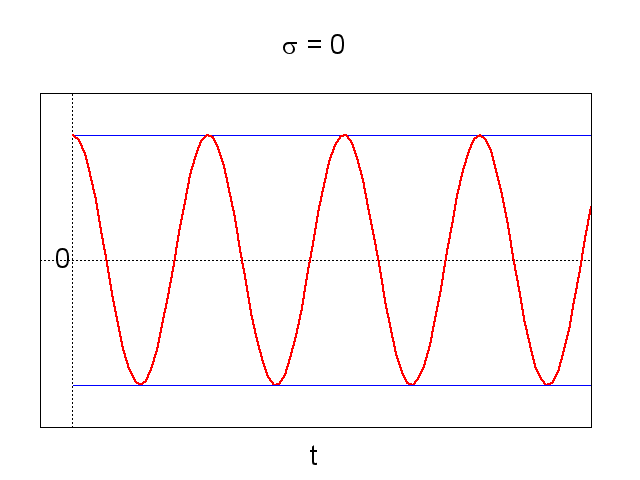
\includegraphics[width=5cm, height=4cm]{plot/andamento_t/poli_complessi1_2}
		\end{subfigure}
		\begin{subfigure}{0.3\textwidth}
			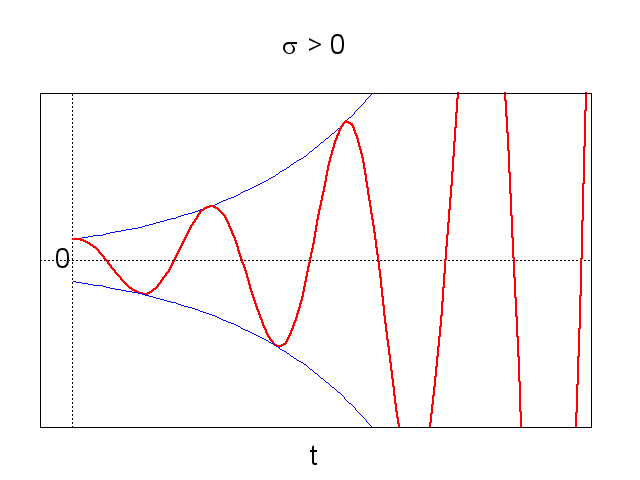
\includegraphics[width=5cm, height=4cm]{plot/andamento_t/poli_complessi1_3}
		\end{subfigure}
	\end{figure}\\
	%2
	\begin{figure}[h!]
		\[ \aLapl{ \frac{c}{(s-p)^2} + \frac{c^*}{(s-p^*)^2} }{ D t e^{\sigma t} \cos (wt + \phi) } \]
		\centering
		\begin{subfigure}{0.3\textwidth}
			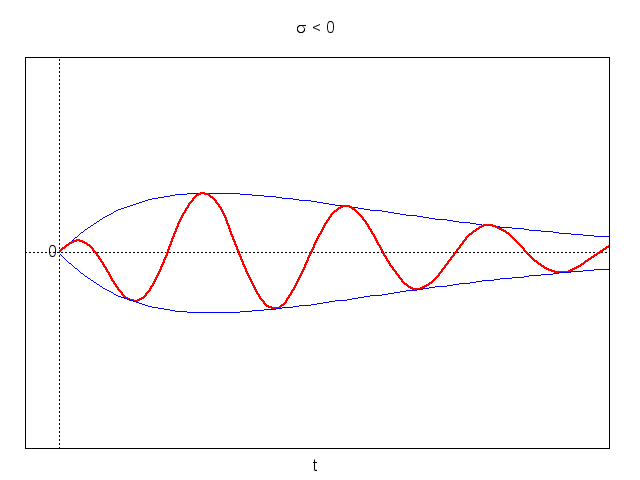
\includegraphics[width=5cm, height=4cm]{plot/andamento_t/poli_complessi2_1}
		\end{subfigure}
		\begin{subfigure}{0.3\textwidth}
			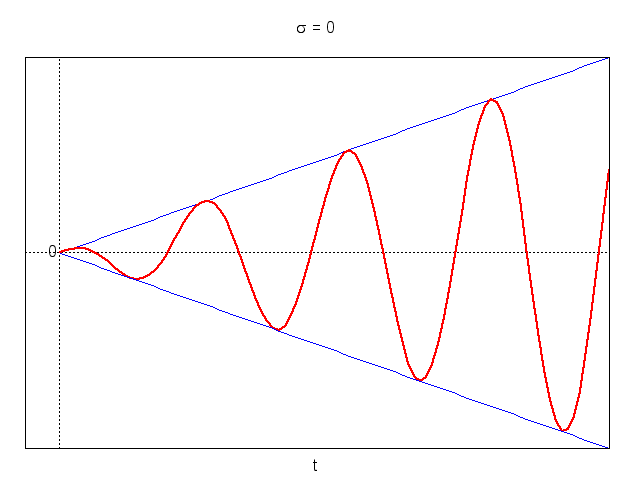
\includegraphics[width=5cm, height=4cm]{plot/andamento_t/poli_complessi2_2}
		\end{subfigure}
		\begin{subfigure}{0.3\textwidth}
			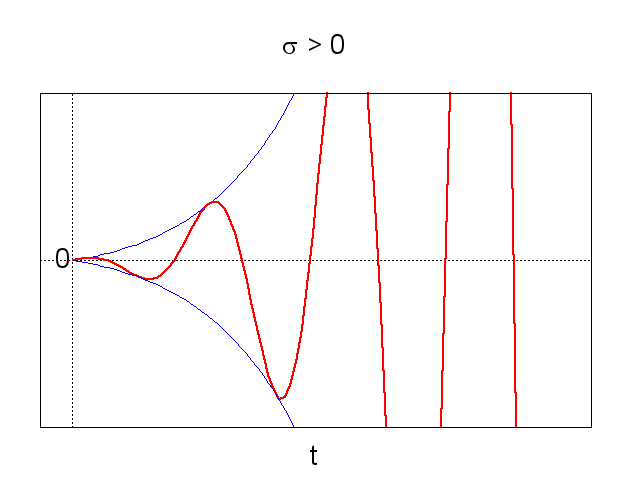
\includegraphics[width=5cm, height=4cm]{plot/andamento_t/poli_complessi2_3}
		\end{subfigure}
	\end{figure}\\
	%3
	\begin{figure}[h!]
		\[ \aLapl{ \frac{c}{(s-p)^n} + \frac{c^*}{(s-p^*)^n} }{ D \frac{1}{(n-1)!} t^n e^{\sigma t} \cos (wt + \phi) } \]
		\centering
		\begin{subfigure}{0.3\textwidth}
			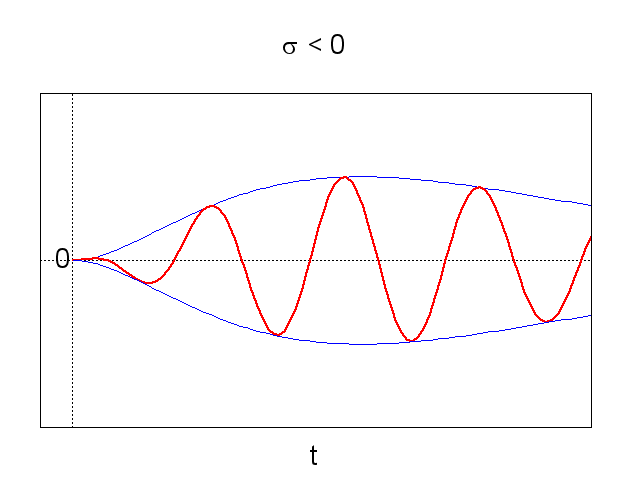
\includegraphics[width=5cm, height=4cm]{plot/andamento_t/poli_complessi3_1}
		\end{subfigure}
		\begin{subfigure}{0.3\textwidth}
			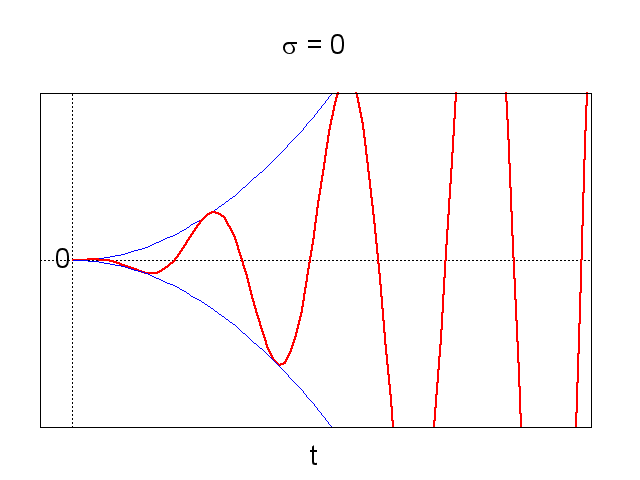
\includegraphics[width=5cm, height=4cm]{plot/andamento_t/poli_complessi3_2}
		\end{subfigure}
		\begin{subfigure}{0.3\textwidth}
			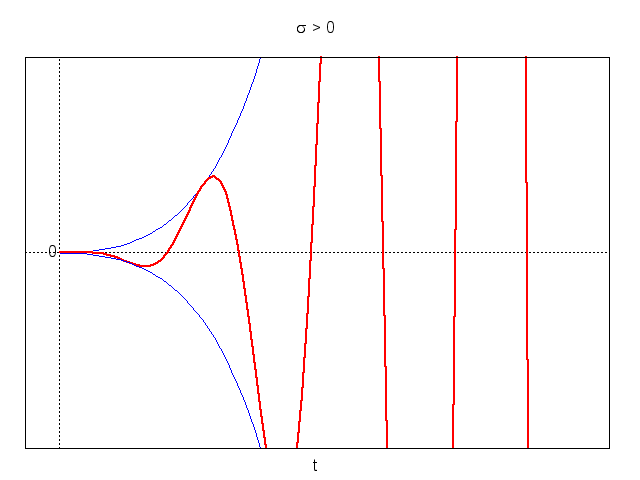
\includegraphics[width=5cm, height=4cm]{plot/andamento_t/poli_complessi3_3}
		\end{subfigure}
	\end{figure}
	%
	\section{Teorema del valore iniziale}
	\[ f(0^+) = \lim\limits_{s \rightarrow +\infty} s F(s) \]
	Questo teorema non richiede particolari ipotesi, ma nel caso delle funzioni razionali non strettamente proprie $ (m \geq n) $ bisogna applicarlo sul resto della divisione.
	\subsection{Esempio: funzione razionale non strettamente propria}
	\[ F(s) = \frac{s+1}{s-1} \]
	Se applicassimo direttamente il teorema, otterremmo un risultato sbagliato:
	\[ f(0^+) = \lim\limits_{s \rightarrow +\infty}s \frac{s+1}{s-1} = +\infty \]
	In realt\'{a} dobbiamo prima calcolare il resto della divisione tra polinomi:
	\[ F(s) = \frac{s+1}{s-1} = \frac{s-1+1+1}{s-1} = \frac{s-1}{s-1} + \frac{2}{s-1} = 1 + \frac{2}{s-1} \]
	\[ f(0^+) = \lim\limits_{s \rightarrow +\infty} s \frac{2}{s-1} = 2 \]
	%
	\section{Teorema del valore finale}
	Sia $ f(t) $ una funzione Laplace-trasformabile con trasformata F(s).\\
	\[ f_\infty = \lim\limits_{t \rightarrow \infty} f(t) \qquad \Rightarrow \qquad f_\infty = \lim\limits_{s \rightarrow 0} s F(s) \]
	Nel caso di poli complessi, l'antitrasformata oscilla attorno a un valore e quindi il teorema non \'{e} applicabile perch\'{e} il limite non esiste. Se per\'{o} tutti i poli non hanno $ \re{p} > 0 $, allora il teorema \'{e} interpretabile come "valore medio asintotico".
	\subsection{Esempio: non applicabile}
	\[ F(s) = \frac{2}{s^2+4} \quad \text{i poli sono:}\ p = \pm 2j \]
	\[ f(t) = \sin(2t) \cdot 1(t) \]
	Il teorema non \'{e} applicabile perch\'{e} la funzione oscilla. Se comunque calcolassi quel limite ottengo:
	\[ \lim\limits_{s \rightarrow 0} s F(s) = \lim\limits_{s \rightarrow 0} \frac{2s}{s^2 + 4} = 0 \]
	%
	\subsection{Esempio: non applicabile}
	\[ F(s) = \frac{1}{s^2-1} = \frac{A}{s+1} + \frac{B}{s-1} \]
	Non si pu\'{o} applicare il teorema perch\'{e} uno dei due poli \'{e} positivo.
	%
	\subsection{Esempio: applicabile}
	\[ F(s) = \frac{1}{s+1} \quad p = -1 \]
	\[ f_\infty = \lim\limits_{s \rightarrow 0} \frac{s}{s+1} = 0 \]
	%
	%esercizi
	\section{Esercizi}
	\begin{mdframed}[style=Exercise]
		\begin{Exercise}[title={Poli reali multipli, poli complessi semplici}, difficulty=2]
			\[
				F(s) = \frac{s^3+s^2+14s-27}{s^4-4s^3+13s^2-36s+36}
			\]
			
			Per fattorizzare il denominatore cerchiamo le sue radici attraverso Ruffini. Con $ 2 $ il denominatore si annulla, quindi dividiamo il polinomio per $ (s-2) $:
			\[ 
				\begin{array}{ccccc|l}
					s^4 & -4s^3 & +13s^2 & -36s & +36 & s-2  \\ \cline{6-6}
					s^4 & -2s^3 &        &      &     & s^3-2s^2+9s-18  \\ \cline{1-2}
					//  & -2s^3 & +13s^2 & -36s & +36 &   \\ 
						& -2s^3 & +4s^2  &      &     &   \\ \cline{2-3} 
						& //    & 9s^2   & -36s & +36 &   \\ 
						& 	    & 9s^2   & -18s &     &   \\ \cline{3-4}
						&       & //     & -18s & +36 &   
				\end{array}
			\]
			\[ 
				Den(s) = (s-2)(s^3-2s^2+9s-18) = (s-2) \big[ s^2(s-2) + 9(s-2) \big] = (s-2)^2 (s^2+9)
			\]
			\[ 
				\begin{cases}
					p_1 = 2
					\\
					n_1=2
				\end{cases}
				\qquad
				\begin{cases}
					p_{2} = + 3j
					\\
					n_{2} = 1
				\end{cases}
				\qquad
				\begin{cases}
					p_{3} = - 3j
					\\
					n_{3} = 1
				\end{cases}
			\]
			\[
				F(s) = c_{11} \frac{1}{s-2} + c_{12} \frac{1}{(s-2)^2} + c_{21} \frac{1}{s-3j} + c_{31} \frac{1}{s+3j}
			\]
			
			$ c_{11} $ potrebbe essere nullo, mentre mi aspetto che $ c_{21} \neq 0 $, altrimenti non potrebbe esistere il fattore $ (s-2)^2 $ nel denominatore.
			
			Per calcolare i residui dei poli reali usiamo la formula \ref{residuo}:
			\begin{itemize}
				\item 
					$ c_{11} \quad q=1 \quad n_1=2 $
					\begin{align*}
						c_{11} &= \frac{1}{(2-1)!} \lim\limits_{s \rightarrow p_1} \der{}{s} (s-2)^2 F(s) = \lim\limits_{s \rightarrow 2} \der{}{s} \left( \frac{s^3+s^2+14s-27}{s^2+9} \right) =
						\\
						&= \lim\limits_{s \rightarrow 2} \frac{(3s^2+2s+14)(s^2+9)-(s^3+s^2+14s-27)2s}{(s^2+9)^2} = 2
					\end{align*}
				\item 
					$ c_{12} \quad q=2 \quad n_1=2 $
					\[
						c_{12} = \dfrac{1}{(2-2)!}\lim\limits_{s \rightarrow 2} \der{^{2-2}}{s^{2-2}} \frac{s^3+s^2+14s-27}{s^2+9} = 1
					\]
			\end{itemize}
			Per calcolare i residui dei poli complessi, la formula precedente conduce a calcoli complicati. \'{E} meglio ricavarli uguagliando i polinomi:
			\begin{align*}
				F(s) &= 2 \frac{1}{s-2} + \frac{1}{(s-2)^2} + A \frac{3}{s^2+9} + B \frac{s}{s^2+9}
				\\
				&= \frac{2(s-2)(s^2+9)+(s^2+9)+3A(s-2)^2+Bs(s-2)^2}{(s-2)^2(s^2+9)} =
				\\
				&= \frac{2s^3+18s-4s^2-36+s^2+9+3As^2-12As+12A+Bs^3-4Bs^2+4Bs}{(s-2)^2(s^2+9)} =
				\\
				&= \frac{(B+2)s^3 + (3A-4B-3)s^2 + (4B-12A+18)s + (12A-27)}{(s-2)^2(s^2+9)}
			\end{align*}
			Abbiamo un sistema ridondante di 4 equazioni in 2 incognite:
			\[ 
				\begin{cases}
					B+2=1
					\\
					3A-4B-3=1
					\\
					4B-12A+18=14
					\\
					12A-27=-27
				\end{cases}\qquad
				\begin{cases}
					B=-1
					\\
					A=0
				\end{cases}
			\]
			\[
				F(s) = \dfrac{2}{s-2} + \dfrac{1}{(s-2)^2} - \dfrac{s}{s^2+9}
			\]
			Quindi si pu\'{o} facilmente ricavare l'antitrasformata:
			\[
				f(t) = \big[ 2e^{2t} + t e^{2t} - \cos(3t) \big] \cdot 1(t)
			\]
		\end{Exercise}
	\end{mdframed}

	\begin{mdframed}[style=Exercise]
		\begin{Exercise}[title={Poli reali multipli, poli complessi semplici}, difficulty=2]
			\[
				F(s) = \frac{8s^3+33s^2+42s+52}{s^5+6s^4+21s^3+26s^2}
			\]
			Fattorizziamo il denominatore:
			\[
				Den(s) = s^2(s^3+6s^2+21s+26)
			\]
			Usiamo il teorema di Ruffini per fattorizzare il polinomio di terzo grado:
			\[ 
				\begin{array}{c|ccc|c}
						& 1 & 6  & 21 & 26  \\ 
					-2 	&   & -2 & -8 & -26 \\ \cline{1-5}
						& 1 & 4  & 13 & 0
				\end{array} 
			\]
			\[
				Den(s) = s^2(s+2)(s^2+4s+13)
			\]
			Le soluzioni del polinomio di secondo grado si possono trovare:
			\begin{itemize}
				\item 
					completamento dei quadrati
					\[
						s^2+4s+4-4+13 = (s+2)^2+9 \quad \Rightarrow \quad \sigma=-2 \quad w=3
					\]
				\item
					formula risolutiva delle equazioni di secondo grado
					\[
						s = \frac{-4 \pm \sqrt{16-52}}{2} = 2 \pm 3j \quad \Rightarrow \quad \sigma=-2 \quad w=3
					\]
			\end{itemize}
			\[
				\begin{cases}
					p_1 = 0\\
					n_1 = 2
				\end{cases}
				\qquad
				\begin{cases}
					p_2 = -2\\
					n_2 = 1
				\end{cases}
				\qquad
				\begin{cases}
					p_3 = 2-3j\\
					n_3 = 1
				\end{cases}
				\qquad
				\begin{cases}
					p_3 = 2+3j\\
					n_3 = 1
				\end{cases}
			\]
			\[
				F(s) = c_{11} \frac{1}{s} + c_{12} \frac{1}{s^2} + c_{21} \frac{1}{s+2} + A \frac{3}{[(s+2)^2+9]} + B \frac{s+2}{[(s+2)^2+9]}
			\]
			\smallskip
			Calcoliamo $ c_{11}, c_{12}, c_{21} $ con la formula dei residui:
			\begin{itemize}
				\item $ c_{11}: \qquad p_1=0 \quad n_1=2 \quad q=1 $
				\begin{align*}
					c_{11} &= \frac{1}{(2-1)!} \lim\limits_{s \rightarrow 0} \der{}{s} s^2F(s) =	\lim\limits_{s \rightarrow 0} \der{}{s} \frac{8s^3+33s^2+42s+52}{s^3+6s^2+21s+26} = \\
					\intertext{quando $ s \rightarrow 0 $ ci interessano solo i termini noti}
					&= \lim\limits_{s \rightarrow 0} \frac{(\dots + 42)(\dots + 26)-(\dots+21)(\dots+52)}{(\dots+26)^2} = \frac{42 \cdot 26 - 21 \cdot 52}{26^2} = 0
				\end{align*}
				\item $ c_{12}: \qquad p_1=0 \quad n_1=2 \quad q=2 $
				\[ c_{12}= \lim\limits_{s \rightarrow 0} s^2F(s) = \lim\limits_{s \rightarrow 0} \frac{\dots + 52}{\dots + 26} = 2 \]
				\item $ c_{21}: \qquad p_1=-2 \quad n_1=1 \quad q=1 $
				\[ c_{21} = \lim\limits_{s \rightarrow -2} (s+2)F(s) = \lim\limits_{s \rightarrow -2} \frac{8s^3+33s^2+42s+52}{s^4+4s^3+13s^2} = 1\]
			\end{itemize}
			\smallskip
			Calcoliamo $ A $ e $ B $ attraverso il sistema:
			\begin{align*}
				&F(s) = \frac{2}{s^2} + \frac{1}{s+2} + A \frac{3}{(s+2)^2+9} + B \frac{s+2}{(s+2)^2+9} =
				\\
				&= \frac{2(s+2)[s^2+4s+13] + s^2[s^2+4s+13] + 3As^2(s+2) + B(s+2)s^2(s+2)}{s^2(s+2)[(s+2)^2+9]} =
				\\
				&= \frac{2s^3 + 8s^2 + 26s + 4s^2 + 16s + 52}{s^2(s+2)[(s+2)^2+9]} +
				\\
				&\qquad + \dfrac{s^4 + 4s^3 + 13s^2 \quad+\quad 3As^3+6As^2 \quad+\quad Bs^4+4Bs^3+4Bs^2}{s^2(s+2)[(s+2)^2+9]} =
				\\
				\intertext{poich\'{e} ho 2 incognite mi servono solo 2 equazioni: posso ignorare le altre}
				&= \frac{(B+1)s^4 + (3A+4B+6)s^3 + \dots}{s^2(s+2)[(s+2)^2+9]}
			\end{align*}
			\[
				\begin{cases}
					B+1=0\\
					3A-4+6=8
				\end{cases}\qquad 
				\begin{cases}
					B=-1\\
					A=2
				\end{cases}								
			\]
			\[
				\Rightarrow\quad F(s) = \frac{2}{s^2} + \frac{1}{s+2} + 2 \frac{3}{[(s+2)^2+9]} - \frac{s+2}{[(s+2)^2+9]}
			\]
			Quindi otteniamo:
			\[
				f(t) = \big( 2t + e^{-2t} + 2e^{-2t}\sin3t - e^{-2t} \cos3t \big) \cdot 1(t)
			\]
		\end{Exercise}
	\end{mdframed}

	\begin{mdframed}[style=Exercise]
		\begin{Exercise}[title={Poli reali semplici, poli complessi multipli}, difficulty=3]
			\[
				F(s) = \frac{2s^4-6s^3+22s^2-18s+16}{(s+1)[(s-1)^2+4]^2}
			\]
			\[
				\begin{cases}
					p_1 = -1\\
					n_1 = 1 
				\end{cases}\quad
				\begin{cases}
					p_2 = 1 - 2j\\
					n_2 = 2
				\end{cases}\quad
				\begin{cases}
					p_3 = 1 + 2j\\
					n_3 = 2
				\end{cases}
			\]
			\[
				F(s) = c_{11} \frac{1}{s+1} + A \frac{2}{[(s-1)^2+4]} + B \frac{s-1}{[(s-1)^2+4]} + C \frac{4(s-1)}{[(s-1)^2+4]^2} + D \frac{(s-1)^2-4}{[(s-1)^2+4]^2}
			\]
			
			A e B possono essere nulli; C e D possono essere nulli, ma non contemporaneamente:
			\[
				c_{11} = \lim\limits_{s \rightarrow -1} (s+1)F(s) = \frac{2+6+22+18+16}{64} = 1
			\]
			Ancora dobbiamo trovare $ A, B, C, D $ quindi ci servono 4 equazioni. Per semplificare i calcoli:
			\begin{align*}
				R(s) &= F(s) - \frac{1}{s+1} = \frac{2s^4-6s^3+22s^2-18s+16}{(s+1)[(s-1)+4]^2} - \frac{1}{s-1} =
				\\
				&= \frac{2s^4-6s^3+22s^2-18s+16\ -\ [(s-1)+4]^2}{(s+1)[(s-1)+4]^2} =
				\\
				&= \dots = \frac{s^4-2s^3-8s^2+2s-9}{(s+1)[(s-1)+4]^2} = \frac{s^3-3s^2+11s-9}{[(s-1)+4]^2}
			\end{align*}
			\[
				\Rightarrow \qquad F(s) = \frac{1}{s+1} + \frac{s^3-3s^2+11s-9}{[(s-1)+4]^2}
			\]
			Adesso riscriviamo $ F(s) $ senza considerare il termine $ \frac{1}{s-1} $:
			\begin{align*}
				&A \frac{2}{[(s-1)^2+4]} + B \frac{s-1}{[(s-1)^2+4]} + C \frac{4(s-1)}{[(s-1)^2+4]^2} + D \frac{(s-1)^2-4}{[(s-1)^2+4]^2} =
				\\
				&= \frac{[2A+B(s-1)][s^2-2s+5] + 4C(s-1) + D[(s-1)^2-4]}{[(s-1)+4]^2} =
				\\
				&= \frac{Bs^3 + (2A+3B+D)s^2 + (10A-5B-4C-2D)s + (10A-5B-4C-3D)}{[(s-1)+4]^2}
			\end{align*}
			Uguagliamo i polinomi e ricaviamo le incognite:
			\[ 
				\begin{cases}
					B = 1\\
					2A + 3 + D = -3\\
					-4A + 7 + 4C - 2D = 11\\
					10A - 5 - 4C - 3D = -9
				\end{cases} \quad
				\begin{cases}
					B=1\\
					-2A=D+6\\
					6A-5D=0\\
					-2A+2C-D=2
				\end{cases} \quad
			\]
			\[
				\begin{cases}
					B=1\\
					-2A=D+6\\
					6A-5D=0\\
					D+6+2C-D=2
				\end{cases} \quad
				\begin{cases}
					A=-\frac{15}{8}\\
					B=1\\
					C=-2\\
					D=-\frac{9}{4}
				\end{cases} \quad
			\]
			Quindi otteniamo:
			\[
				f(t) = [1 \cdot e^{-t} -\frac{15}{8} e^t \sin2t + 1 \cdot \cos2t -2 \cdot t e^t \sin2t -\frac{9}{4} t e^t \cos2t] \cdot 1(t)
			\]
		\end{Exercise}
	\end{mdframed}
\end{document}